\documentclass{article}

\usepackage{graphicx}
\usepackage[T1]{fontenc}
\usepackage[polish]{babel}
\usepackage[utf8]{inputenc}
\usepackage{float}
\usepackage{wrapfig}
\usepackage{csvsimple}
\usepackage{booktabs}

\newcommand{\companyName}{Nintendo Co. Ltd } % Szybka zmiana w razie zmiany danych
\newcommand{\samplesFrom}{02.01.2019 }
\newcommand{\samplesTo}{13.03.2023}
\graphicspath{{../Images/}}
\title{Wskaźnik Giełdowy MACD}
\date{27.03.2023}
\author{Krzysztof Napiórkowski}


\begin{document}
\maketitle
    \section{Wstęp}
    Celem projektu jest implementacja wskaźnika giełdowego MACD oraz przedstawienie algorytmu wykorzystującego go do zautomatyzowania kupna i sprzedarzy akcji. 
    Do realizacji wykorzystałem język Python z bibliotekami: pandas, numpy oraz matplotlib.
    Wskaźnik jest wykonany dla \companyName, dane pobrane z Yahoo finance.

    \section{Analiza zadania}
    
    \subsection{Dane}
    Dane wskaźnika dotyczą notowania spółki w okresie od \samplesFrom do \samplesTo. \\
    Z przedziału brane było 1000 próbek, w danych mogło brakować niektórych dni. Na potrzeby zadania dane były traktowane jako kolejne dni.
    Średnia krocząca jest obliczana z ceny zamknięcia.

    \begin{figure}[ht]
        \centering
        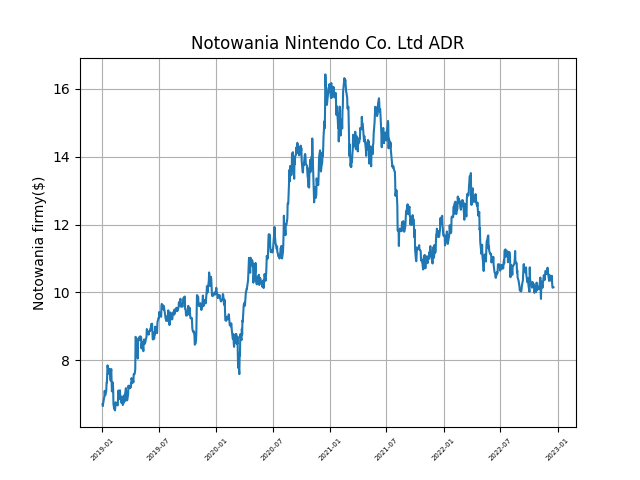
\includegraphics[scale=0.5]{Samples}
        \caption{Notowania spółki \companyName w okresie od \samplesFrom do \samplesTo}
        \label{fig:samples}
    \end{figure}

    \subsection{Podstawa teoretyczna}
    Wskaźnik MACD składa się z dwóch wykresów: MACD oraz linii sygnałowej SIGNAL. 
    Oba opierają się na wykładniczej średniej kroczącej, określonej wzorem: \\
    \begin{equation}
        EMA_{N} = \frac{p_{0} + (1-\alpha)p_{1} + \dots + (1-\alpha)^N p_{N}}{(1-\alpha) + \dots + (1-\alpha)^N}
    \end{equation}
    gdzie: \\ \newline
    $ \alpha = \frac{2}{N - 1} $ \\
    $ N $ - liczba okresów \\
    $ p_{i} $ - wartość danej sprzed $ i $ dni \\

    Składowa MACD jest różnicą $ EMA_{12} - EMA_{26} $ obliczoną w oparciu o dane. Linia sygnałowa SINGAL jest obliczana jako $ EMA_{9} $ ze składowej MACD.

    \subsection{Wykres składowych wskaźnika MACD}
    \begin{figure}[ht]
        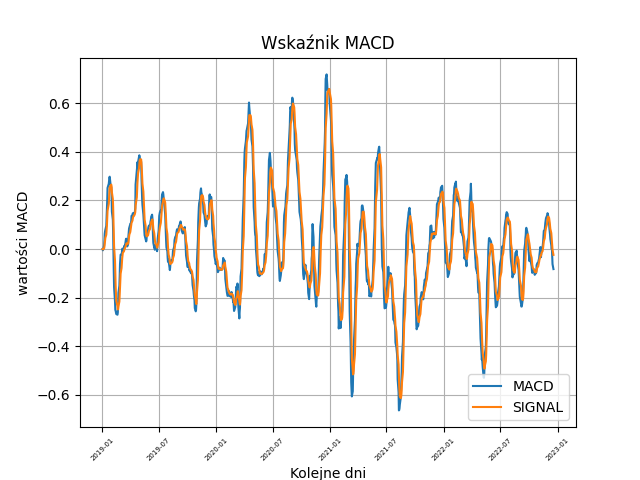
\includegraphics[width=\textwidth]{MACD}
        \caption{wskaźnik MACD dla \companyName}
        \label{fig:macd}
    \end{figure}

    \subsection{analiza wskaźnika MACD}
    Wskaźnik MACD jest wykorzystywany do inwestycji przecięcie lini sygnału przez linię MACD od dołu oznacza zapowiedź trendu wzrostowego i jest sygnałem kupna.
    przecięcie od góry oznacza zapowiedź trendu opadającego i jest sygnałem sprzedaży.
    \begin{figure}[ht]
        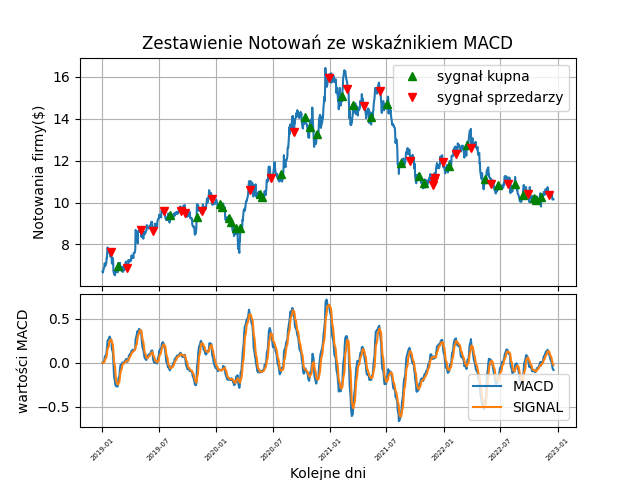
\includegraphics[width=\textwidth]{TradeSignals}
        \caption{Przedstawienie sygnałów zakupu i sprzedarzy na podstawie MACD}
        \label{fig:compare}
    \end{figure}
    
    Jak widać na wykresie w wielu przypadkach sygnał kupna pojawia się za wcześnie i ostatecznie kolejny sygnał sprzedarzy nie przewyższa początkowego.
    Wskaźnik sprawdza się w momencie w którym same notowania rosnął to w takim przypadku dobrze wykrywa momenty kupna i sprzedarzy.  Gdy notowanie spada to wykrywa wzrosty lokalne i daje fałszywe sygnały.


    \newpage
    \section{Algorytm automatyzujący}
    Algorytmu polega na sprzedarzy i kupnie w momencie przecięcia się MACD oraz SIGNAL oraz określenia trendu zwyżkującego, bądź zniżkującego, poprzez sprawdzanie wartości MACD.
    dla porównania przedstawiam 3 wersje: kupno i sprzedarz po 1 akcji, sprzedarz i kupno wszyskiego możliwego oraz sprzedarz i kupno 50\% możliwych akcji.

    \subsection{sprzedarz po 1 akcji:}
    \begin{table}[ht]
        \centering
        \begin{tabular}{rrrr}
\toprule
 Dzień &     Kapitał &  Akcje &  Zarobek \\
\midrule
   100 &  999.898000 &      0 &    -0.10 \\
   200 & 1000.068000 &      0 &     0.07 \\
   300 &  953.538001 &      5 &    -7.54 \\
   400 &  934.496001 &      7 &    14.37 \\
   500 &  906.890002 &      9 &    48.33 \\
   700 &  909.774001 &      9 &    11.56 \\
   900 &  932.772002 &      7 &    11.17 \\
   999 &  901.744002 &     10 &     3.24 \\
\bottomrule
\end{tabular}

        \caption{Zestawienie zarobku dla wyznaczonych dni}
    \end{table}
    Metoda sprzedarzy i kupna po jednej akcji nie okazała się zbytnio opłacalna, choś udało nam się zarobić około \$20 to w skali 5 lat nie jest to znaczący zarobek.

    \subsection{sprzedarz po 50\% posiadanych akcji oraz kupnie 50\% możliwych:}
    \begin{table}[ht]
        \centering
        \begin{tabular}{rrrr}
\toprule
 Dzień &    Kapitał &  Akcje &  Zarobek \\
\midrule
   100 & 900.958010 &     18 &    59.86 \\
   200 & 929.452017 &     15 &    63.88 \\
   300 &  41.478033 &    109 &  -110.07 \\
   400 & 355.706043 &     81 &   279.92 \\
   500 & 129.310070 &     96 &   638.05 \\
   700 & 875.156028 &     49 &   429.35 \\
   900 & 921.752061 &     42 &   392.15 \\
   999 & 728.024083 &     60 &   337.02 \\
\bottomrule
\end{tabular}

        \caption{Zestawienie zarobku dla wyznaczonych dni}
    \end{table}
    Metoda najbardziej skuteczna, choć ciągle nie na tyle opłacalna aby ryzykować na prawdziwej giełdzie.
    

    \subsection{sprzedarz wszystkich akcji oraz kupno wszystkich możliwych:}
    \begin{table}[ht]
        \centering
        \begin{tabular}{rrrr}
\toprule
 Dzień &     Kapitał &  Akcje &  Zarobek \\
\midrule
   100 &  985.414034 &      0 &   -14.59 \\
   200 & 1003.094042 &      0 &     3.09 \\
   300 &    4.584079 &    104 &  -185.88 \\
   400 &    2.016122 &    104 &   188.66 \\
   500 &   10.392183 &     98 &   550.56 \\
   700 & 1422.450043 &      0 &   422.45 \\
   900 & 1394.298164 &      0 &   394.30 \\
   999 & 1355.294215 &      0 &   355.29 \\
\bottomrule
\end{tabular}

        \caption{Zestawienie zarobku dla wyznaczonych dni}
    \end{table}
    Chociaż okazała się najbardziej skuteczna to również jest najbardziej podatna na fałszywe sygnały. Więc jej skuteczność jest najbardziej zależna od szczęśćia.
    
    \subsection{wykrsy zysku aktualny kapitał + cena akcji disiaj * ilość akcji - początkowy kapitał}
    \begin{figure}[ht]
        \centering
        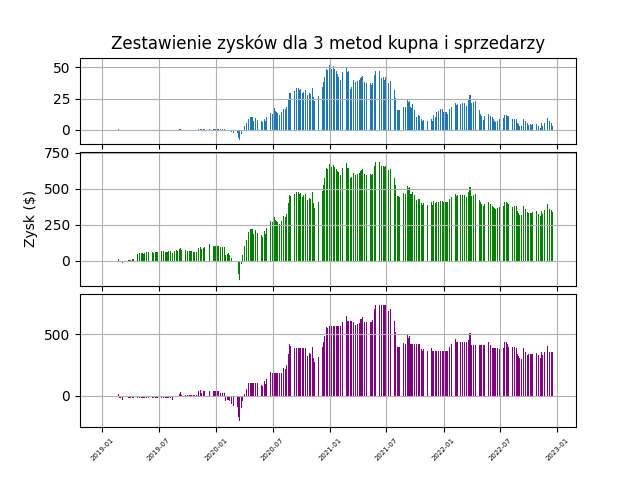
\includegraphics[scale=0.6]{MethodComparision}
        \caption{Zestawienie zarobków dla trzech podanych metod handlu}
    \end{figure}    

    Na Rysunku 4 widać dokładny podział na wykresach. W pierwszej części widać znikomy, bądź nawet zerowy zysk. Widoczny zysk ukazujes się dopiero po jakimś czasie. 
    Może być to spowodowane, że wskaźnik MACD jest opóźniony oraz słabym wzrostem notowania w tej części.
    
    \section{Podsumowanie i wnioski}
    Krzywa MACD jest bardzo przydatnym narzędziem do badania notowań giełdowych ale przez opóźnienie w notowaniu może skutkować w stratę, szczególnie dla inwestycji krótkoterminowych. 

    \section{Źródła}
    dane - https://finance.yahoo.com/quote/NTDOY/history?p=NTDOY\\
    https://en.wikipedia.org/wiki/MACD\\
    https://www.edukacjagieldowa.pl/gieldowe-abc/analiza-techniczna/narzedzia-analizy-technicznej/krzywa-macd/\\
    instrukcja do zadania\\

\end{document}
